\documentclass[12pt]{article}
\usepackage[margin=2.5cm]{geometry}
\usepackage{enumerate}
\usepackage{amsfonts}
\usepackage{amsmath}
\usepackage{fancyhdr}
\usepackage{amsmath}
\usepackage{amssymb}
\usepackage{amsthm}
\usepackage{mdframed}
\usepackage{graphicx}
\usepackage{subcaption}
\usepackage{adjustbox}
\usepackage{listings}
\usepackage{xcolor}
\usepackage{booktabs}
\usepackage[utf]{kotex}
\usepackage{hyperref}

\definecolor{codegreen}{rgb}{0,0.6,0}
\definecolor{codegray}{rgb}{0.5,0.5,0.5}
\definecolor{codepurple}{rgb}{0.58,0,0.82}
\definecolor{backcolour}{rgb}{0.95,0.95,0.92}

\lstdefinestyle{mystyle}{
    backgroundcolor=\color{backcolour},
    commentstyle=\color{codegreen},
    keywordstyle=\color{magenta},
    numberstyle=\tiny\color{codegray},
    stringstyle=\color{codepurple},
    basicstyle=\ttfamily\footnotesize,
    breakatwhitespace=false,
    breaklines=true,
    captionpos=b,
    keepspaces=true,
    numbers=left,
    numbersep=5pt,
    showspaces=false,
    showstringspaces=false,
    showtabs=false,
    tabsize=1
}

\lstset{style=mystyle}

\pagestyle{fancy}
\renewcommand{\headrulewidth}{0.4pt}
\lhead{Team Treehouse}
\rhead{Querying Relational Databases Part 4 Notes}

\begin{document}
\title{Querying Relational Databases Part 4 Notes}
\author{Team Treehouse}
\maketitle

\bigskip

\section{Join Queries}

\bigskip

\begin{itemize}
    \item Joins two tables into one
    \item Is used in tables with one to one relationship

    \begin{center}
    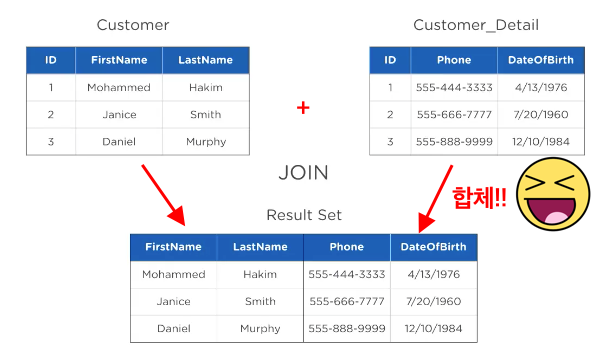
\includegraphics[width=0.8\linewidth]{images/part_4_notes_1.png}
    \end{center}
\end{itemize}

\bigskip

\section{Inner Joins}

\begin{center}
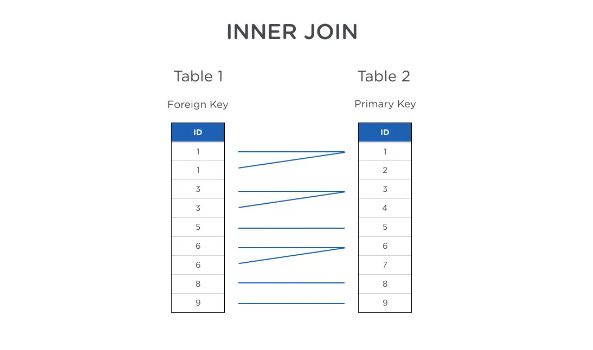
\includegraphics[width=\linewidth]{images/part_4_notes_3.png}
\end{center}

\bigskip

\begin{itemize}
    \item Is most common type of JOIN
    \item Is used for joining one to many relationships
    \item \textbf{Syntax:} SELECT \textit{columns name} FROM \textit{table 1 (many) name}
    INNER JOIN \textit{table 2 (one) name} ON \textit{table 1 name}.\textit{column name} = \textit{table 1 name}.\textit{column name};

    \bigskip

    \underline{\textbf{Example:}}

    \bigskip

    \begin{lstlisting}[language=SQL]
    SELECT mk.MakeName = md.ModelName FROM make AS mk
    INNER JOIN model AS md ON mk.MakeId = md.MakeId;
    \end{lstlisting}

    \bigskip

    \begin{center}
    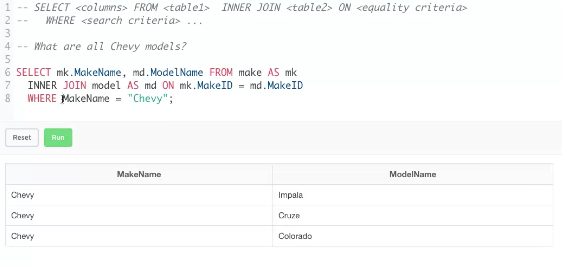
\includegraphics[width=0.8\linewidth]{images/part_4_notes_2.png}
    \end{center}
\end{itemize}


\end{document}